\subsection{Modellierung der Systemdynamik} \label{Dynamik_sec}
In dem folgenden Abschnitt werden die Bewegungsgleichungen mit Hilfe des Lagrange Formalismus hergeleitet. Aus diesen Gleichung kann im Anschluss eine Zustandsraumdarstellung aufgestellt werden, welche als Grundlage für den Reglerentwurf dient.

\begin{figure}[h]
\centering
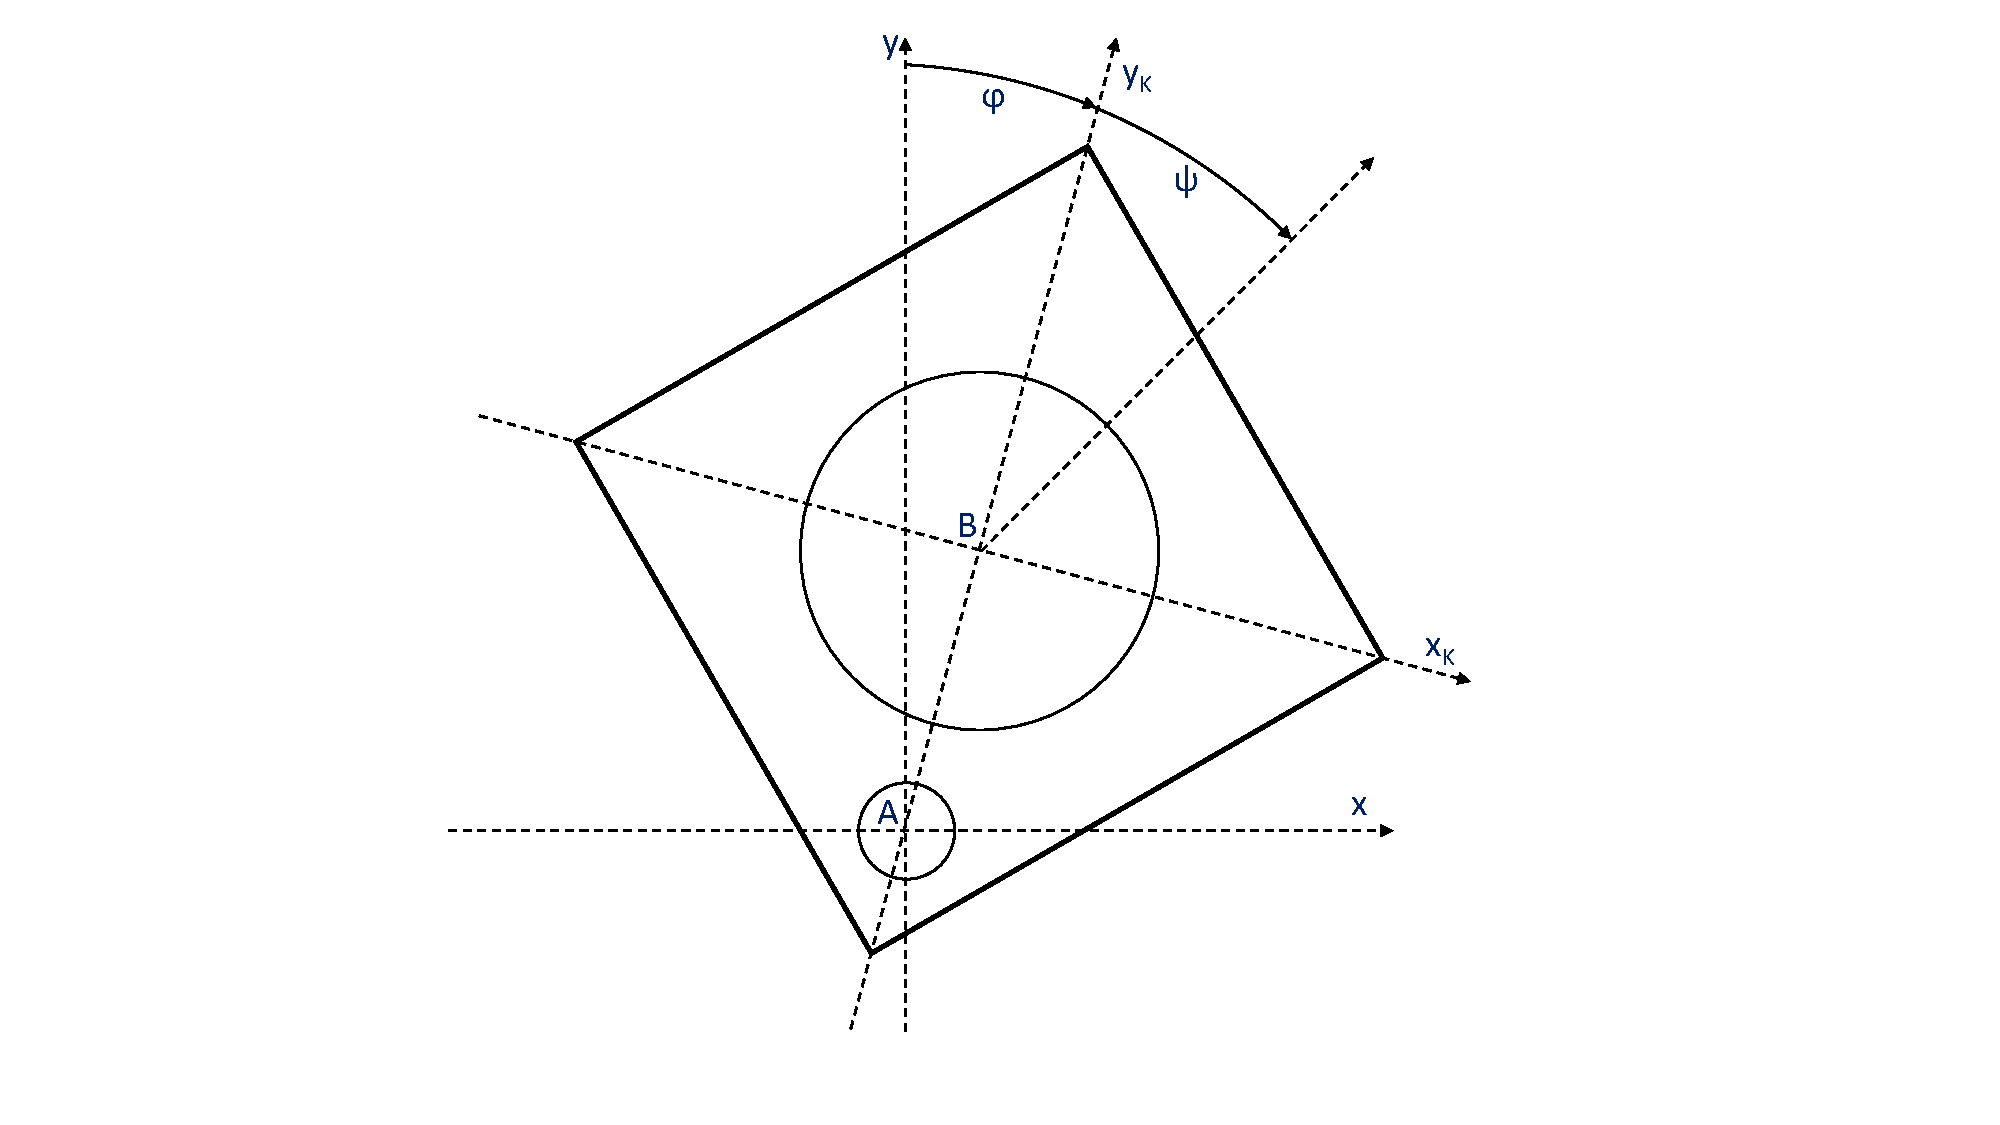
\includegraphics[width=\linewidth]{MechZeichnung1D}
\caption{Mechanischer Aufbau, Quelle: eigene Darstellung}
\end{figure}

Der Prototyp besteht aus einem starren Körper der in $A$ auf einer Achse gelagert ist. In $B$ ist eine Schwungmasse über einen Motor mit dem Körper verbunden. Somit verfügt das Gesamtsystem über zwei Freiheitsgrade, welche durch die generalisierten Koordinaten 

\begin{equation}
q_1 = \varphi \hspace{35pt} q_2 = \psi
\end{equation}

beschrieben werden. Der Winkel $\varphi$ wird von den Achsen $y$ und $y_K$ eingeschlossen. Der Winkel beschreibt die rotatorische Verschiebung der Schwungmasse zu dem Körper. Die folgenden Größen beschreiben die weiteren physikalischen Gegebenheiten des Systems.\newline

\begin{table}[h]
\centering
\begin{tabular}{|c|c|}
\hline
	\textbf{Variable} & \textbf{Erklärung} \\ \hline
	$q_1 = \varphi$ & Ausfallwinkel des Körpers \\ \hline
	$q_2 = \psi$ & Winkel zwischen Schwungmasse und Körper \\ \hline
	$A$ & Drehpunkt des Körpers \\ \hline
	$B$ & Drehpunkt des Schwungrades \\ \hline
	$l_{AB}$ & Abstand zwischen $A$ und $B$ \\ \hline
	$l_{AC}$ & Abstand zwischen $A$ und dem Schwerpunkt des Körpers \\ \hline
	$m_K$ & Masse des Körpers \\ \hline
	$m_R$ & Masse des Schwungrades \\ \hline
	${\theta}^A_K$ & Massenträgheitsmoment des Körper um $A$ \\ \hline
	${\theta}^B_R$ & Massenträgheitsmoment der Schwungmasse um $B$ \\ \hline
	$C_{\varphi}$ & Dynamischer Reibkoeffizient des Körpers in $A$ \\ \hline
	$C_{\psi}$ & Dynamischer Reibkoeffizient des Schwungrades in $B$ \\ \hline
	$T_M$ & Drehmoment des Motor \\ \hline
\end{tabular}
\end{table}

\newpage
Um die Bewegungsgleichungen des Systems zu ermitteln wird der Lagrange Formalismus verwendet. Dieser basiert auf der Lagrange-Funktion $L$, welche die Differenz der kinetischen Energie $T$ und der potenziellen Energie $V$ des Systems beschreibt.

\begin{equation}
T = \frac{1}{2}[({\theta}^A_K + m_R \cdot {l_{AB}}^2) {\dot{\varphi}}^2 + {\theta}^B_R(\dot{\varphi}+\dot{\psi})^2]
\end{equation}
\begin{equation}
V = g(m_R \cdot l_{AB} + m_K \cdot l_{AC})cos(\varphi)
\end{equation}
\begin{equation}
L = T - V = \frac{1}{2}[({\theta}^A_K + m_R \cdot {l_{AB}}^2) {\dot{\varphi}}^2 + {\theta}^B_R(\dot{\varphi}+\dot{\psi})^2] - g(m_R \cdot l_{AB} + m_K \cdot l_{AC})cos(\varphi)
\end{equation}

In dem System wirken unterschiedliche Kräfte und Momente, welche nach dem Lagrange-Formalismus als generalisierte Kraftkomponenten $Q_i$ dargestellt werden können. Das Ziel hiervon ist es, die Summe der Kräfte, bzw. deren verrichtete Arbeit, in Komponenten zu zerteilen, welche in Richtung der generalisierten Koordinaten wirken. Die generalisierten Kraftkomponenten können nach der folgenden Formel berechnet werden, wobei $F_j$ die verschiedenen Kräfte bzw. Momente und $r_j$ eine Verrückung in ihrer Wirkungsrichtung darstellt.
\begin{equation}
Q_i = \sum F_j \cdot \frac{\partial r_j}{\partial q_i} 
\end{equation}
Durch die Gravitation wirkt eine konstante Kraft entgegen der raumfesten y-Koordinate auf den Körper.
\begin{equation}
F_1 \cdot r_1 = -g \cdot (m_K \cdot y_K + m_R  \cdot y_R) = -g \cdot(m_K \cdot l_{AC} + m_R \cdot l_{AB}) \cdot cos(\varphi)
\end{equation}
Durch den Motor und die Reibung in den beiden Lagern entstehen die Drehmomente $T_M$, $M_{R_{\varpi}}$ und $M_{R_{\psi}}$, welche entlang der generalisierten Koordinaten wirken und somit nicht umgeformt werden müssen. Die Reibmomente werden als linear proportional zu der momentanen Winkelgeschwindigkeit modelliert.
\begin{equation}
F_2 \cdot r_2 = T_M \cdot \psi
\end{equation}

\begin{equation}
F_3 \cdot r_3 = M_{R_{\varphi}} \cdot \varphi = (-C_{\varphi} \cdot \dot{\varphi}) \cdot \varphi
\end{equation}

\begin{equation}
F_4 \cdot r_4 = M_{R_{\psi}} \cdot \psi = (-C_{\psi} \cdot \dot{\psi}) \cdot \psi
\end{equation}
Somit können nun die Summe der Kräfte und Momente gebildet werden und daraufhin die generalisierten Kraftkomponenten bestimmt werden.
\begin{equation}
\begin{split}
Q_{\varphi} &= -g \cdot (m_K \cdot l_{AC} + m_R \cdot l_{AB}) \cdot \frac{\partial cos(\varphi)}{\partial \varphi} + T_M \cdot \frac{\partial \psi}{\partial \varphi} + C_{\varphi} \cdot \dot{\varphi} \cdot \frac{\partial \varphi}{\partial \varphi} + C_{\psi} \cdot \dot{\psi} \cdot \frac{\partial \psi}{\partial \varphi} \\
&= g \cdot (m_K \cdot l_{AC} + m_R \cdot l_{AB})\cdot sin(\varphi) - C_{\varphi} \cdot \dot{\varphi}
\end{split}
\end{equation}

\begin{equation}
\begin{split}
Q_{\psi} &= -g \cdot (m_K \cdot l_{AC} + m_R \cdot l_{AB}) \cdot \frac{\partial cos(\varphi)}{\partial \psi} + T_M \cdot \frac{\partial \psi}{\partial \psi} + C_{\varphi} \cdot \dot{\varphi} \cdot \frac{\partial \varphi}{\partial \psi} + C_{\psi} \cdot \dot{\psi} \cdot \frac{\partial \psi}{\partial \psi} \\
&= T_M - C_{\psi} \cdot \dot{\psi}
\end{split}
\end{equation}

Bei dem Prototyp handelt es sich um ein nicht konservatives System, da durch die Reibung mechanische Energie verloren geht und der Motor dem System mechanische Energie zuführt. Da die beiden generalisierten Koordinaten $\varphi$ und $\psi$ voneinander unabhängig sind können aus dem d'Alembert'schen Prinzip zwei Bewegungsgleichungen abgeleitet werden.

\begin{equation}
\frac{d}{dt}\frac{\partial T}{\partial \dot{q}_i}-\frac{\partial T}{\partial q_i} = Q_i
\end{equation}
\begin{equation}
\frac{d}{dt}\frac{\partial T}{\partial \dot{\varphi}}-\frac{\partial T}{\partial \varphi} = Q_{\varphi} 
\end{equation}
\begin{equation}
\label{LG_phi_equation}
({\theta}^A_K + {\theta}^B_R + m_R \cdot l_{AB}^2)\ddot{\varphi} + {\theta}^B_R \cdot \ddot{\psi} - g(m_R \cdot l_{AB} + m_K \cdot l_{AC})sin(\varphi) + C_{\varphi} \cdot \dot{\varphi} = 0
\end{equation}
\begin{equation}
\frac{d}{dt}\frac{\partial T}{\partial \dot{\psi}}-\frac{\partial T}{\partial \psi} = Q_{\psi} 
\end{equation}
\begin{equation}
\label{LG_psi_euqation}
{\theta}^R_B \cdot \ddot{\psi} = T_M - C_{\psi} \cdot \dot{\psi} - {\theta}^B_R \cdot \ddot{\varphi}
\end{equation}
\newpage
Durch Einsetzen von (\ref{LG_psi_euqation}) in (\ref{LG_phi_equation}) ergibt sich die folgende Bewegungsgleichung für die Würfelseite.

\begin{equation}
\label{BG_phi_quation}
\ddot{\varphi} = \frac{g(m_R \cdot l_{AB} + m_K \cdot l_{AC})sin(\varphi) - C_{\varphi} \cdot \dot{\varphi} + C_{\psi} \cdot \dot{\psi} - T_M}{{\theta}^A_K + m_R \cdot l_{AB}^2}
\end{equation}

Die Bewegungsgleichung für die Schwungmasse ergibt sich durch Einsetzen von (\ref{BG_phi_quation}) in (\ref{LG_psi_euqation}).

\begin{equation}
\label{BG_psi_equation}
\ddot{\psi} = \frac{({\theta}^A_K + m_R \cdot l_{AB}^2 + {\theta}^B_R)(T_M - C_{\psi} \cdot \dot{\psi})}{({\theta}^A_K + m_R \cdot {l_{AB}}^2){\theta}^B_R} + \frac{C_{\varphi} \cdot \dot{\varphi} - g(m_R \cdot l_{AB} + m_K \cdot l_{AC})sin(\varphi)}{{\theta}^A_K + m_R \cdot {l_{AB}}^2}
\end{equation}